\section{DQN on Atari}

Now that you have completed your implementation of DQN it is time to train an agent to play Pong using your code. Before we start this section we would also like to provide a kind reminder to \textbf{terminate any unused Azure instances in order to avoid running out of credits}. \\

\textbf{A Brief History of Pong:}

Pong is a table tennis themed arcade game which was officially released by Atari in 1972. At this point in time, Atari consisted of only two people Nolan Bushnell and Allan Alcorn. The creation of the arcade game was assigned to Allan Alcorn, unbeknownst to him it was assigned as a training exercise. Despite initially being set as a training exercise, Pong went on to become an officially released arcade game. The release of Pong was a major success and today it is often touted as being responsible for the rise in popularity of arcade video games.

Fortunately, we will have the opportunity to test the performance of our reinforcement learning agent on this historic game. What's more, we can expect our implementation of DQN to perform at a super human level. Let's get started! \\

\textbf{Simulating Atari Games}:

We will leverage the \href{https://www.gymlibrary.dev/}{gym python package} to simulate the arcade game Pong. In general, the gym package provides a suite of environments within which you may test reinforcement learning algorithms. For details of all the available environments and usage of the gym python package, please consult the official \href{https://www.gymlibrary.dev/}{documentation} for the library. \\

\textbf{Data Preprocessing:}

The Atari environment from Gymnasium (former OpenAI gym) returns observations (or original frames) of size $ (210 \times 160 \times 3) $, the last dimension corresponds to the RGB channels filled with values between $ 0 $ and $ 255 $ (\texttt{uint8}). Following DeepMind's \href{https://storage.googleapis.com/deepmind-media/dqn/DQNNaturePaper.pdf}{paper}, we will apply the following preprocessing to the observations:
\begin{enumerate}[1.]
\item To encode a single frame, we take the maximum value for each pixel color value over the frame being encoded and the previous frame. In other words, we return a pixel-wise max-pooling of the last 2 observations.
\item Convert the encoded frame to grey scale; crop and rescale it to $(80 \times 80 \times 1)$. (See Figure \ref{fig:pong_env})
\end{enumerate}

The above preprocessing is applied to the 4 most recent observations and these encoded frames are stacked together to produce the input (of shape $(80 \times 80 \times 4)$) to the Q-function. Also, for each time we decide on an action, we perform that action for 4 time steps. This reduces the frequency of decisions without impacting the performance too much and enables us to play 4 times as many games while training. You can refer to the \textit{Methods} section of DeepMind's \href{https://storage.googleapis.com/deepmind-media/dqn/DQNNaturePaper.pdf}{paper} for more details. \\

\begin{figure}[H]
\centering
\begin{subfigure}[b]{.4\textwidth}
  \centering
  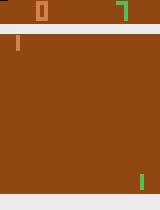
\includegraphics[width=.25\linewidth]{images/pong}
  \caption{Original input $ (210 \times 160 \times 3)$ }
  \label{fig:pong}
\end{subfigure}
\begin{subfigure}[b]{.4\textwidth}
  \centering
  
\includegraphics[width=.25\linewidth]{images/pong_grey}
  \caption{Input after preprocessing $ (80 \times 80 \times 1 ) $}
  \label{fig:pong_grey}
\end{subfigure}
\caption{\texttt{Pong} environment}
\label{fig:pong_env}
\end{figure}

\textbf{Setting up your Virtual Machine}

Follow the instructions in the \href{https://github.com/scpd-proed/XCS234-Handouts/blob/main/Azure/Azure%20Guide.pdf}{Azure Guide} in order to create your vm instance and deploy the assignment code to your vm. Though you will need the GPU to train your model, we strongly advise that you first develop the code locally and ensure that it runs, before attempting to train it on your vm (passing the grader tests and debugging on the test environment should be sufficient). GPU time is expensive and limited. It takes approximately \textbf{8 hours} to train our DQN model. We don't want you to accidentally use all your GPU time for the assignment, debugging your model rather than training and evaluating it. Finally, \textbf{make sure that your VM is turned off whenever you are not using it.}

In order to run the model code on your vm, please run the following command to create the proper virtual environment:

\begin{lstlisting}
$ conda update -n base conda
$ conda env create --file environment_cuda.yml
\end{lstlisting}

\textit{Note: we are using the gpu version of the conda environment file.}

For local development and testing, see the \nameref{intro} for instructions on which environment you should use.

If you wish to monitor your model training in real-time, you may optionally activate tensorboard and port forward the tensorboard outputs on your vm to an available port on your local machine (we strongly recommend that you do). This will enable you to view the tensorboard dashboard and your model training metrics on your local machine in real-time. To get this setup you should first start training your implementation of DQN in order to generate training metrics for tensorboard to plot (or optionally have already trained your implementation and simply wish to visualize the results).

By default tensorboard runs on port 6006. Therefore, we will look to port forward 6006 on your vm to an available port on your local machine using ssh. For this you will need to identify an available port on your local machine. To test if a process is already running on a particular port simply enter the following command in your bash session ~lsof -i : <port_number>~. If this returns a process, you will need to either kill this process or find a new port (don't kill any processes without understanding its purposes and the reprecusions of stopping the process). Once you have established an available port, let's say for example 12345, then run the following command (which will forward vm's port 6006 to your desktop) \textit{from your local machine}:

\begin{lstlisting}
# Run this from your local machine where you run the browser
$ ssh -L 12345:localhost:6006 -p xxxxx student@ml-lab-xxxxxxx.eastus.cloudapp.azure.com
\end{lstlisting}

Where, in the above command, you will need to fill in the sections marked with "x". These values should align with those you regularly use to ssh onto your vm (see \href{https://github.com/scpd-proed/XCS234-Handouts/blob/main/Azure/Azure%20Guide.pdf}{Azure Guide} for further details). You should now be prompted to enter the password you have already setup for your virtual machine. Enter your password and run the following command to start tensorboard:

\begin{lstlisting}
# Run this from vm
$ tensorboard --logdir=<results_folder> --host 0.0.0.0
\end{lstlisting}

Finally, open up a browser on your local machine and visit \textit{http://localhost:12345} to view the tensorboard dashboard. Note that use \textit{http} not \textit{https} for the above command.

\begin{enumerate}[(a)]

	\item \points{7a}

Now we're ready to train on the Atari \texttt{Pong-v0} environment. First, launch linear approximation on pong by running the following command:
\begin{lstlisting}
$ python run.py --config_filename=q7_linear
\end{lstlisting} 
This will train the model for $500,000$ steps and should take approximately an hour. Once training is complete observe the contents of ~results/q7_linear~ and in particular the plot ~scores.png~ (the \href{https://github.com/scpd-proed/XCS234-Handouts/blob/main/Azure/Azure%20Guide.pdf}{Azure Guide} contains details of moving files from the vm to your local machine). 

Using this plot please refer to and answer question 3.1 of the Gradescope online assessment ~A2 (Quiz)~. 


	\item \points{4b}

In this question, we'll train the agent with DeepMind's architecture on the Atari \texttt{Pong} environment. Run the following command to start the training process:
\begin{lstlisting}
$ python run.py --config_filename=q4_dqn
\end{lstlisting}
To speed up training, we have trained the model for 5 million steps (these pretrained weights will be automatically loaded once you run the above command). You are responsible for training it to completion, which should take \textbf{6 hours}. You should get a score of around 12-15 after 4 million total time steps.  As stated previously, the DeepMind paper claims average human performance is $ -3 $. Once your model has fully trained download the following file to your local machine ~src/submission/model.weights~ and include these weights with your code submission to Gradescope. 

\textit{Note: the weights file needs to be in the submission folder for the autograder to read them when you run the grader on your local machine.}


As the training time is roughly 6 hours, you may want to check after a few epochs that your network is making progress.  The following are some training tips:

\begin{itemize}
\item If you terminate your terminal session, any training processes which are running within this session will terminate.  In order to avoid this, you can start a session with Tmux which will persist even if you lose your connection to the vm. See the Azure guide for further details).
\item The evaluation score printed on terminal should start at 6 and increase.
\item The max of the q values should also be increasing.
\item The standard deviation of q shouldn't be too small. Otherwise it means that all states have similar q values.
\item Please find our Tensorboard graphs from one training session below.
\end{itemize}

\begin{figure}[H]
\centering
  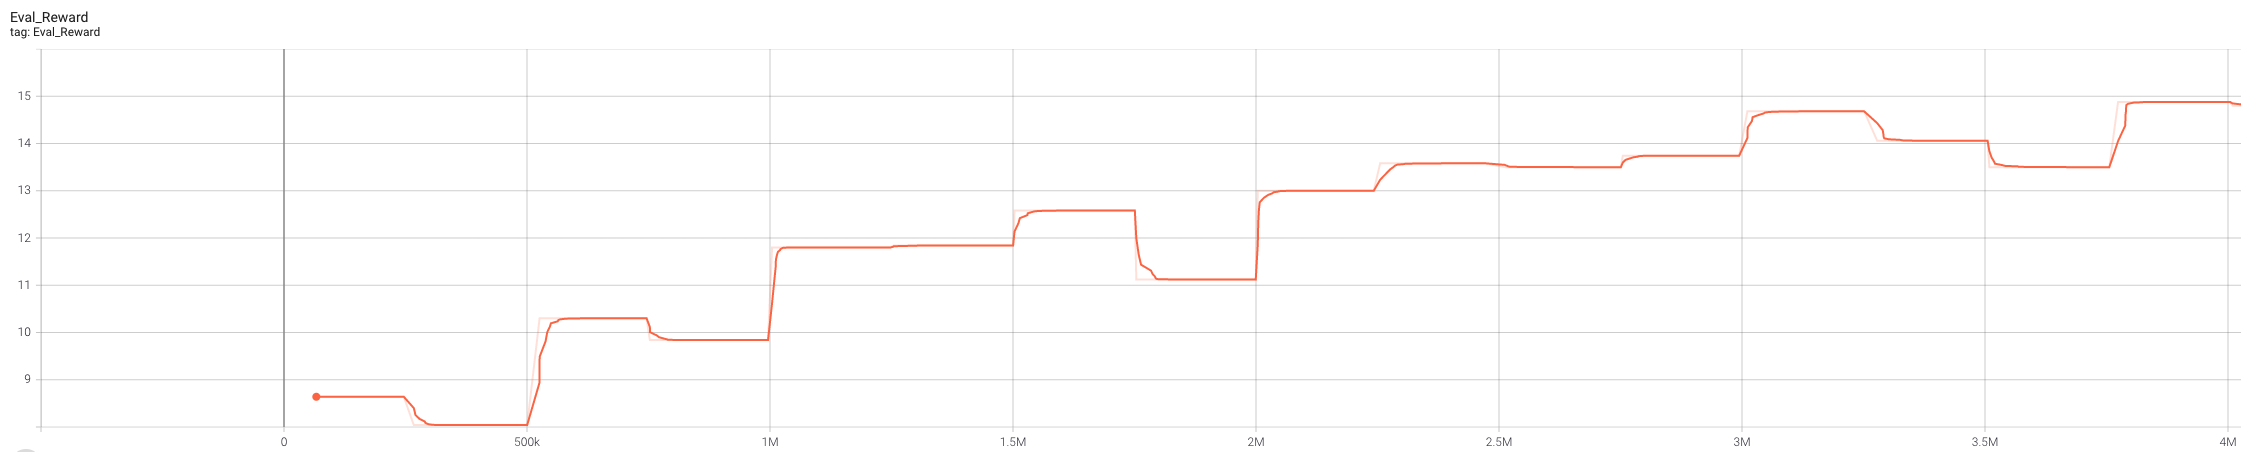
\includegraphics[width=.4\linewidth]{images/Eval_R.png}
  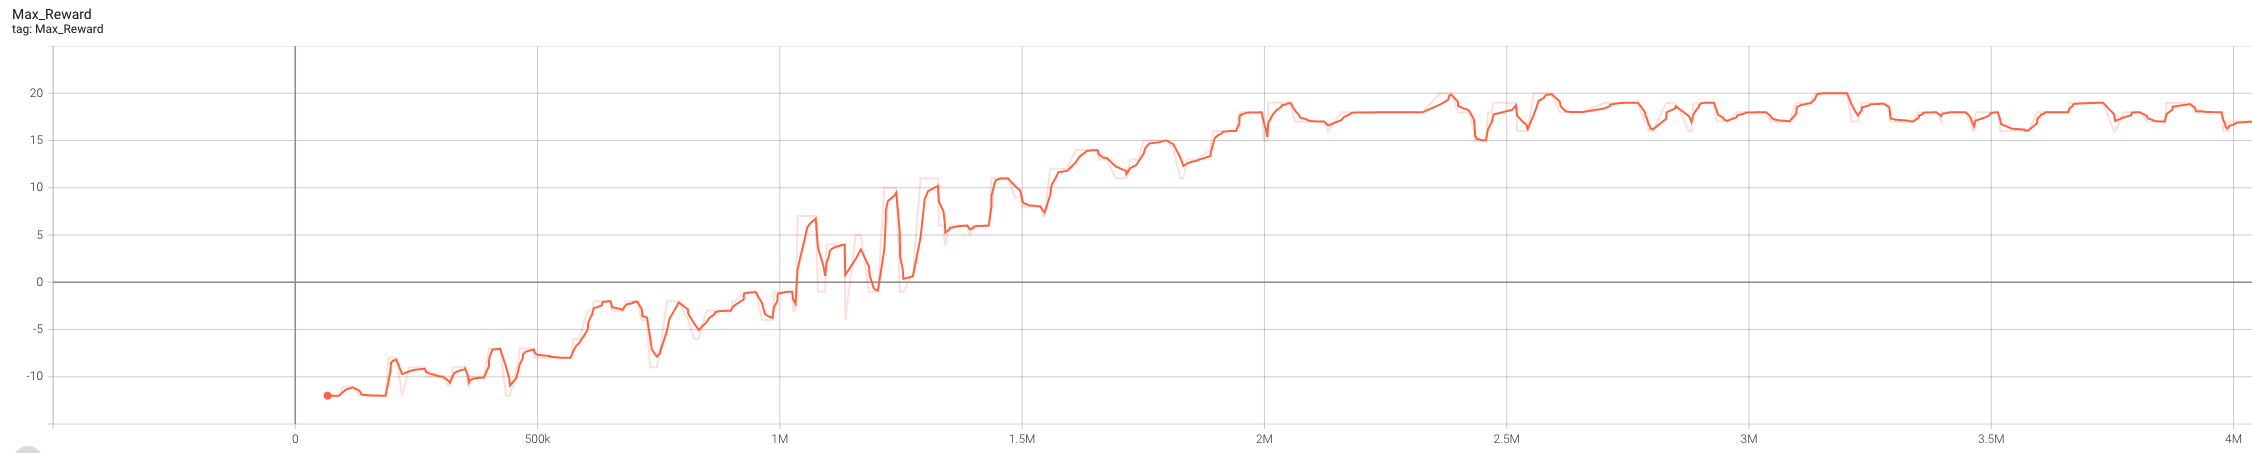
\includegraphics[width=.4\linewidth]{images/Max_R.png}
  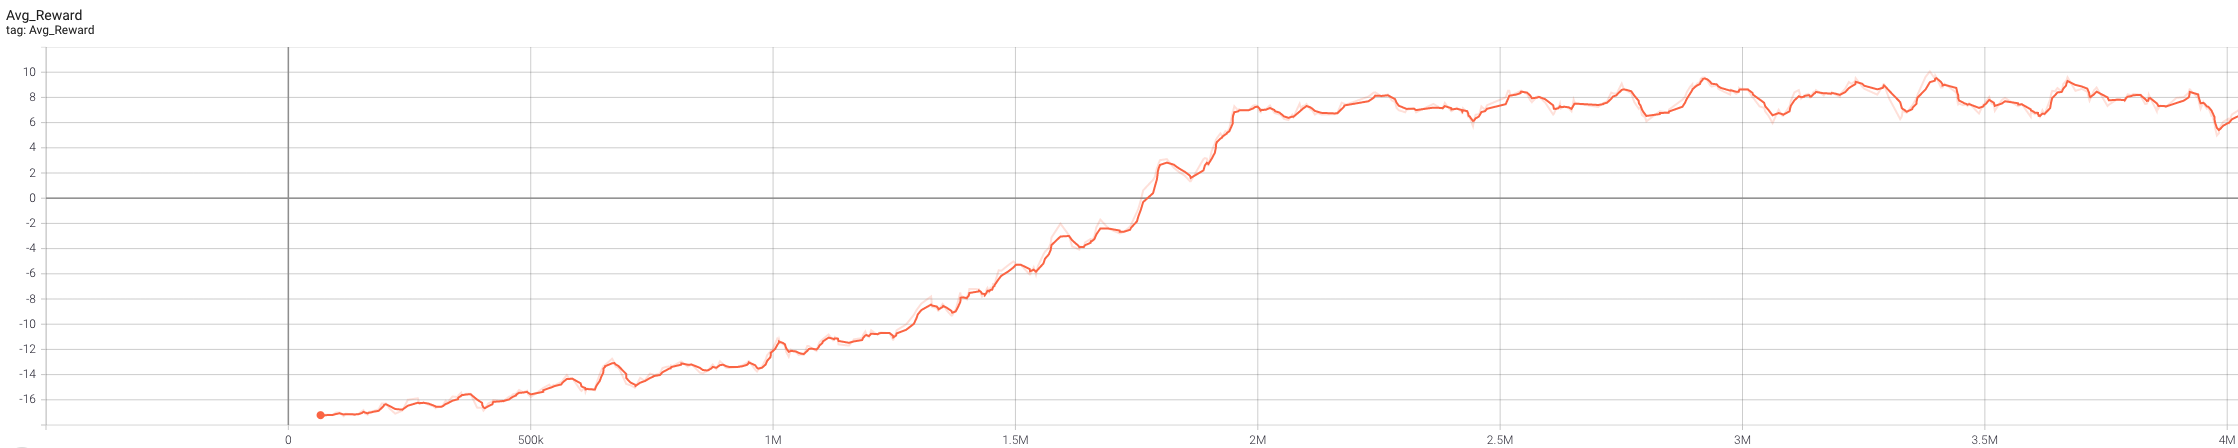
\includegraphics[width=.4\linewidth]{images/Avg_R.png}
  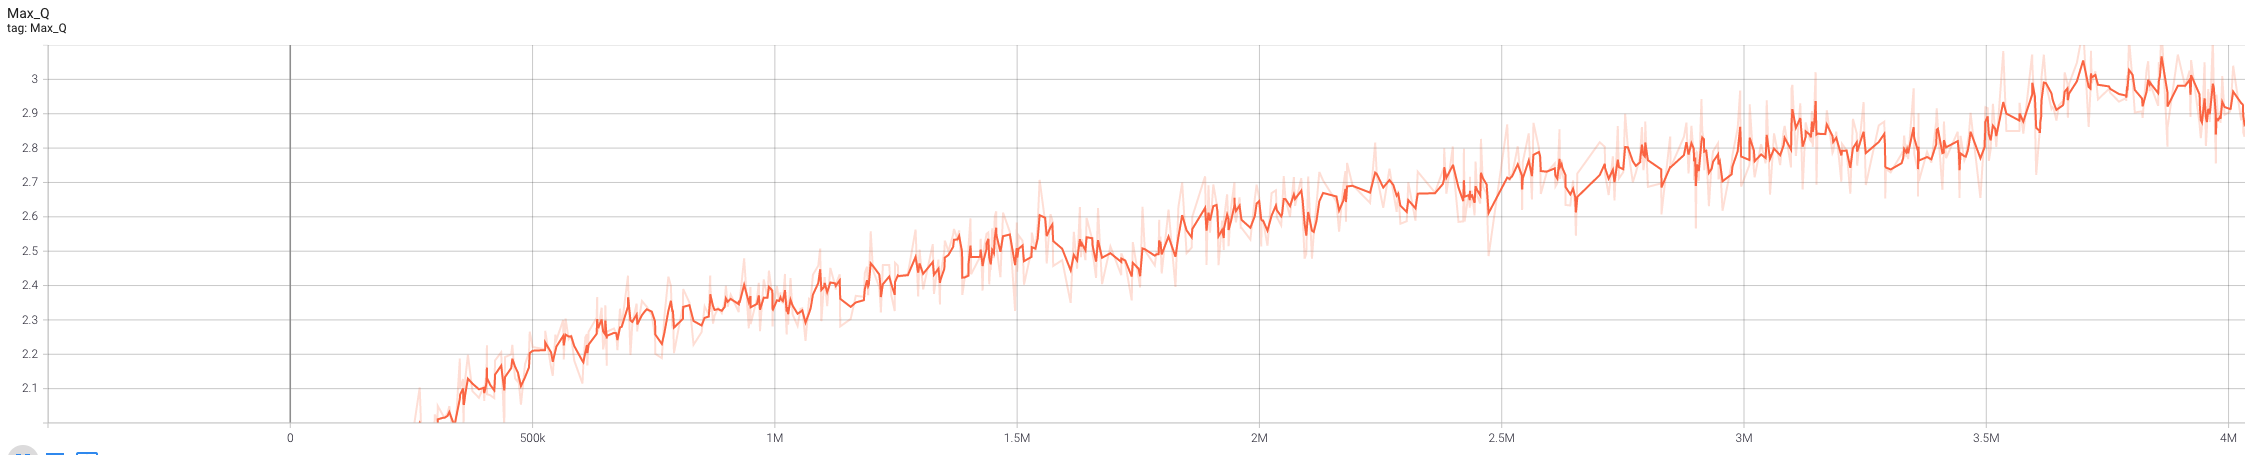
\includegraphics[width=.4\linewidth]{images/Max_Q.png}
\end{figure}

  \item \points{7c}

Please refer to question 3.2 of the Gradescope online assessment ~A2 (Quiz)~.


  \item \points{7d}

Please refer to questions 3.3 of the Gradescope online assessment ~A2 (Quiz)~.


\end{enumerate}
